%%%%%%%%%%%%%%
% LECTURE 19 %
%%%%%%%%%%%%%%
\vspace{1cm}

\noindent\lecture{19}{13/12/2021}

\section{Sistemi a trappola ionica}
A partire da questa sezione focalizzeremo la nostra attenzione sullo studio del controllo e della realizzazione fisica (pratica) di sistemi costituiti da qubit e gate. 

\noindent I sistemi basati sulle cosiddette \textbf{trappole di ioni} sono una tecnologia sperimentale sviluppatasi nel corso degli anni '80. Come già introdotto all'inizio del capitolo, queste apparecchiature sono costituite da un campo elettromagnetico generato da una serie di elettrodi cilindrici che intrappola al proprio interno un gruppo di ioni (solitamente ioni di berillio). Si faccia riferimento alla Figura \ref{fig:ion-trap1} di Pagina \pageref{fig:ion-trap1} per una rappresentazione schematica. A causa della loro particolare disposizione, gli elettrodi generano un potenziale\footnote{I pedici \textbf{dc} e \textbf{rf} significano rispettivamente \textit{direct current} e \textit{radio frequency}.} indipendente dal tempo e uno variabile:
\begin{align*}
    \phi_{\text{dc}} &= k U_0 \left( z^2 - x^2 - y^2 \right) \, , \\
    \phi_{\text{rf}} &= \left( V_0 \cos(\Omega t) + U_0 \right) \left( 1-\frac{x^2-y^2}{R^2} \right) \, .
\end{align*}
È possibile mostrare che l'effetto di questi potenziali è quello di creare un'hamiltoniana con il seguente potenziale armonico
\begin{equation*}
    H = \sum_{i=1}^N \frac{M}{2} \left( \omega_x^2 x_i^2 + \omega_y^2 y_i^2 + \omega_z^2 z_i^2 \right) + \sum_{j>i} \frac{e^2}{4 \pi \varepsilon_0 \abs{\vec{x}_i - \vec{x}_j}} \, ,
\end{equation*}
dove $N$ è il numero di ioni intrappolati dal campo e $M$ la loro massa (il secondo termine è repulsivo). Per realizzare un tale setup si sceglie una direzione privilegiata (per convenzione $z$) tale per cui $\omega_x, \omega_y \gg \omega_z$, in questo modo l'effetto che si ottiene è che gli ioni cercano di allinearsi solamente lungo $z$, ossia la direzione in cui sono "accesi" i modi vibrazionali (lungo $x$ e $y$ sono soppressi). Diagonalizzando esplicitamente un'hamiltoniana della forma precedente si ricava che la frequenza minore è associata al moto del centro di massa del sistema: la frequenza minima corrisponde quindi al movimento rigido degli ioni lungo $z$. 

\noindent Per gli scopi del QC vorremmo essere in grado di indirizzare e manipolare a piacimento gli stati quantistici del sistema. Innanzitutto è necessario lavorare a temperature molto basse, ossia $k T \ll \hbar \omega_z$ (molto più piccole del primo stato eccitato), perché nessuno dei modi vibrazionali lungo $x$ o $y$ deve essere eccitato. Non entriamo nei dettagli\footnote{Ad esempio viene effettuato il cosiddetto \textbf{Doppler cooling}, il quale sfrutta il fatto che, per effetto Doppler, la frequenza degli ioni in movimento rispetto al laser cambi a seconda del verso del moto. In questo modo solamente gli ioni che si dirigono verso il laser possono assorbire fotoni, al contrario invece di quelli che si muovono in direzione contraria.}, tuttavia ci limitiamo a sottolineare che questa procedura di raffreddamento viene attuata per mezzo di opportuni laser. In aggiunta ai laser è necessario costruire le cosiddette \textbf{sidebands}: si eccitano i livelli energetici interni degli stati degli ioni in modo tale che si possano etichettare gli stati utilizzando anche i modi vibrazionali. In generale entrambe queste procedure possono essere realizzate sperimentalmente con il seguente risultato: il primo stato eccitato quantistico corrisponde all'oscillazione del centro di massa del sistema lungo $z$ con frequenza $\omega_z$. 

\noindent Spesso i modi vibrazionali che possono essere eccitati sono comunemente detti \textbf{fononi}. Il moto (oscillazione) del centro di massa è il primo elemento su cui si basano i sistemi a trappola ionica e può essere descritto in maniera del tutto analoga ad un oscillatore armonico: come nella \eqref{x_a_adag}, la quantizzazione è effettuata promuovendo la coordinata spaziale ad operatore
\begin{equation*}
    \hat{z} = z_0 (\hat{a} + \hat{a}^\dag) \, , \quad \text{dove} \quad z_0 = \sqrt{\frac{\hbar}{2 \omega M N}} \, .
\end{equation*}

\noindent Il secondo ingrediente che si aggiunge ai modi vibrazionali sono gli stati atomici degli ioni: solitamente si scelgono opportunamente gli ioni in maniera tale che si riescano a isolare esplicitamente due livelli energetici dello spettro rispetto a tutti gli altri; in questo modo è possibile codificare in questi livelli un qubit, ma soprattutto, essendo gli stati separati dal resto dello spettro, sono facilmente controllabili dai laser.  Per ridurre al minimo la probabilità di transizione $\ket{1} \to \ket{0} $ a seguito dell'emissione spontanea si cercano degli stati eccitati che presentano una vita media molto lunga, come ad esempio alcuni ioni con stati eccitati metastabili. Un'altra scelta è quella di sfruttare la struttura iperfine dei livelli energetici degli ioni (dovuta all'interazione tra gli spin dei nucleoni e degli elettroni esterni): visto che l'ampiezza di decadimento per emissione spontanea \`e $\Gamma \sim \omega^3$, questi livelli sono molto più stabili di altri livelli energetici atomici.  

\noindent Come già mostrato nella Figura \ref{fig:ion-trap2}, per gli scopi del QC i qubit sono codificati in ciascuno degli ioni (si ottiene un array di qubit) utilizzando entrambi gli stati precedenti: un generico stato è quindi descritto da entrambi i modi, quelli vibrazionali (fononi) e quelli energetici. Per quanto riguarda i fononi si utilizzano due livelli: $\ket{0}$, ossia nessun fonone, e il suo stato eccitato $\ket{1}$, un fonone; vedremo a breve che utilizzando questi stati è possibile codificare un qubit extra, detto \textbf{bus qubit}. 

\noindent Per interagire con un sistema così generato si utilizzano delle opportune radiazioni elettromagnetiche generate da laser. Queste radiazioni presentano un comportamento classico, quindi consideriamo l'accoppiamento tra qubit e campo esterno classico oscillante della Sezione \ref{sec:qubit_campo_em_classico} (notare che gli operatori $\hat{a}$ e $\hat{a}^\dag$ fanno riferimento ai modi vibrazionali, non al campo quantizzato). Consideriamo un solo ione: l'interazione con il campo è descritta dall'accoppiamento $\vec{d} \cdot \vec{E}$, quindi l'hamiltoniana non è altro che la \eqref{H_couple}, ossia
\begin{equation}\label{da_espandere_kz}
    \hat{H} = \Omega \hat{\sigma}_1 \cos \left( k z - \omega t + \phi \right) \, .
\end{equation}
In questo contesto $kz \simeq k z_0 = 2\pi \frac{z_0}{\lambda}$ e $k z_0 \equiv \eta$ è detto \textbf{parametro di Lamb-Dicke}, il quale misura il rapporto tra l'ampiezza dell'oscillazione dei modi vibrazionali del qubit e la lunghezza d'onda della radiazione. Per assicurare che $kz$ sia circa costante sul qubit dobbiamo stare attenti alle due scale del problema:
\begin{enumerate}
    \item Dato che la grandezza dei qubit è quella degli ioni allora vorremmo che la lunghezza d'onda dei laser ($\lambda$) sia molto più grande delle scale atomiche. 
    
    \item Per la presenza dei modi vibrazionali lungo $z$ dobbiamo richiedere che $\lambda$ sia molto più grande delle oscillazioni lungo $z$. 
\end{enumerate}
\noindent Quando le precedenti sono verificate possiamo assumere che $kz \ll 1$, ma non completamente trascurabile, in modo tale da poter effettuare un'espansione perturbativa della \eqref{da_espandere_kz}:
\begin{equation*}
    \hat{H} = \Omega \hat{\sigma}_1 \cos \left( -\omega t + \phi \right) - \Omega k z \hat{\sigma}_1 \sin \left( -\omega t + \phi \right) + \order{(kz)^2} \, ;
\end{equation*}
inserendo gli operatori e trascurando i termini di ordine superiore avremo
\begin{equation}\label{hams_I_II}
    \begin{aligned}
        \hat{H} &= \underbrace{\frac{\Omega}{2} (\hat{\sigma}_+ + \hat{\sigma}_-) \left( e^{-i(\omega t - \phi)} + e^{i(\omega t - \phi)}  \right)}_{\hat{H}_{(I)}} + \\
        &\quad + \underbrace{i \frac{\Omega}{2} \eta (\hat{\sigma}_+ + \hat{\sigma}_-) (\hat{a} + \hat{a}^\dag) \left( e^{-i(\omega t - \phi)} - e^{i(\omega t - \phi)}  \right)}_{\hat{H}_{(II)}} \, ,
    \end{aligned}
\end{equation}
dove abbiamo distinto i due termini di $\hat{H}$ perché tra poco vedremo che contribuiranno in modo differente. Assumiamo di lavorare in un regime in cui la frequenza del laser sia sintonizzata su entrambe le frequenze in gioco, ossia quella della differenza in energia dei livelli del qubit e la frequenza dei modi vibrazionali. Per questo possiamo utilizzare nuovamente la RWA perché sappiamo che solo i termini in risonanza contribuiscono. Innanzitutto, l'hamiltoniana libera e l'operatore $\hat{U}$ con cui effettuiamo la rotazione saranno ($\hbar = 1$)
\begin{equation*}
    \hat{H}_0 = -\frac{\omega_q}{2} \hat{\sigma}_3 + \omega_z (\hat{a}^\dag \hat{a}) \, , \quad \Rightarrow \quad \hat{U} = e^{i \hat{H}_0 t} \, ;
\end{equation*}
facendo uso delle \eqref{RWA_ops_trans} (chiaramente in questo contesto $\omega_c \equiv \omega_z$) possiamo facilmente scrivere l'hamiltoniana ruotata della \eqref{S_eq_rotated_state}: come sappiamo ogni operatore ottiene un fattore di fase e l'idea è quella di tenere solamente i termini in risonanza e trascurare tutti gli altri per tempi molto lunghi. 

\begin{figure}[H]
	\centering	
	\subfloat[][\label{subfig:levels_ion_trap1} ]{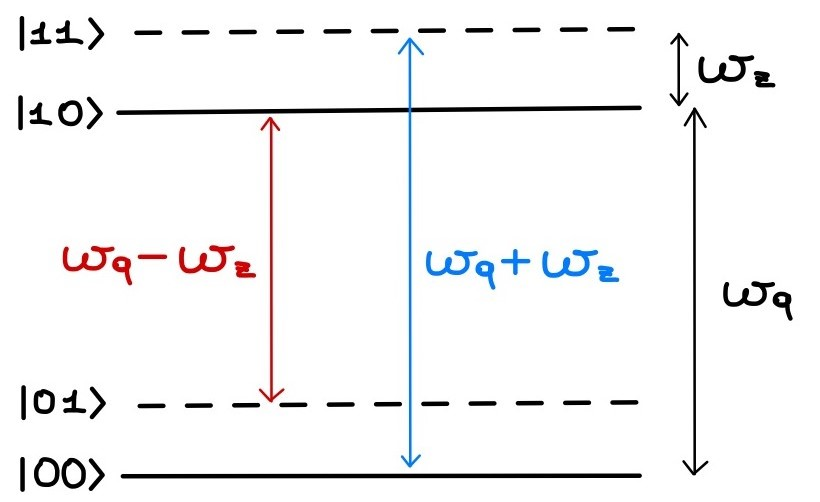
\includegraphics[scale=.45,keepaspectratio]{images/levels_ion_trap1}} \\
	\subfloat[][\label{subfig:levels_ion_trap2} ]{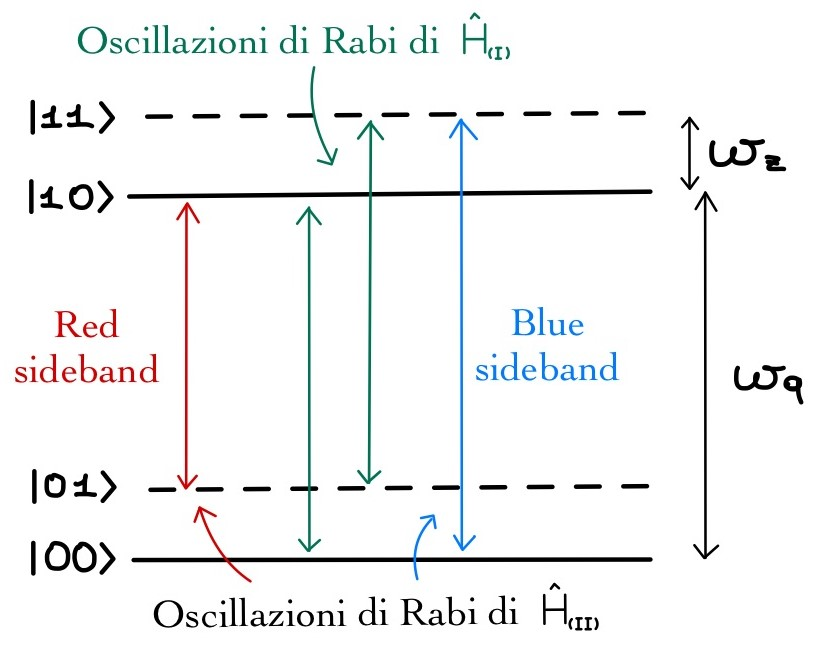
\includegraphics[scale=.45,keepaspectratio]{images/levels_ion_trap2}}
	\caption{(\ref{subfig:levels_ion_trap1}) Suddivisione dei livelli energetici degli ioni in un sistema a trappola ionica. Le frequenze $\omega_q - \omega_z$ e $\omega_q + \omega_z$ sono dette \textbf{red sideband} e \textbf{blue sideband} rispettivamente.  (\ref{subfig:levels_ion_trap2}) Oscillazioni di Rabi prodotte dai termini delle hamiltoniane $\hat{H}_{(I)}$ e $\hat{H}_{(II)}$. Notare che per la red sideband contribuiscono gli operatori $\hat{\sigma}_- \hat{a}$ ($\ket{01} \to \ket{10}$) e $\hat{\sigma}_+ \hat{a}^\dag$ ($\ket{10} \to \ket{01}$); mentre per la blue sideband contribuiscono $\hat{\sigma}_+ \hat{a}$ ($\ket{11} \to \ket{00}$) e $\hat{\sigma}_- \hat{a}^\dag$ ($\ket{00} \to \ket{11}$).}
    \label{fig:levels_ion_trap}
\end{figure}

\noindent Ci sono molti termini che possono contribuire a seconda della frequenza del laser. L'idea nei sistemi a trappola ionica è quella di utilizzare una radiazione che possa accomodare 4 differenti frequenze. Innanzitutto etichettiamo gli stati del sistema con la notazione $\ket{nm}$, dove $n$ è il livello energetico del qubit e $m$ il modo di oscillazione vibrazionale (fonone). Tenendo conto della Figura \ref{subfig:levels_ion_trap1} vorremmo utilizzare le 4 frequenze $\pm \omega_q \pm \omega_z$ e $\pm \omega_q$ (quest'ultimo permette le oscillazioni $\ket{0m} \leftrightarrow \ket{1m}$).

\noindent Scriviamo i termini che "sopravvivono" dalla RWA nelle due hamiltoniane $\hat{H}_{(I)}$ e $\hat{H}_{(II)}$:
\begin{align}
    \hat{H}_{(I)} &= \frac{\Omega}{2} \left( \hat{\sigma}_+ e^{i(\omega t - \phi)} + \hat{\sigma}_- e^{-i(\omega t - \phi)} \right) \label{H_I_Rabi} \\
    \hat{H}_{(II)} &= i \frac{\eta \Omega}{2} \left( -\hat{\sigma}_+ \hat{a}^\dag e^{i(\omega t - \phi)} + \hat{\sigma}_- \hat{a} e^{-i(\omega t - \phi)} \right) + \label{H_II_sideband} \\
    &\quad + i \frac{\eta \Omega}{2} \left( -\hat{\sigma}_+ \hat{a} e^{i(\omega t - \phi)} + \hat{\sigma}_- \hat{a}^\dag e^{-i(\omega t - \phi)} \right) \, , \notag
\end{align}
dove nella \eqref{H_I_Rabi} abbiamo assunto $\omega \sim \omega_q$ e nella \eqref{H_II_sideband} si ha $\omega \sim \omega_q - \omega_z$ nella prima riga e $\omega \sim \omega_q + \omega_z$ nella seconda (notare che $\omega$ in queste due righe è scelto appositamente per annullare le fasi derivanti dalla \eqref{RWA_ops_trans}). Come evidente dal disegno in Figura \ref{subfig:levels_ion_trap2}, $\hat{H}_{(I)}$ genera oscillazioni di Rabi tra $\ket{0 m} \leftrightarrow \ket{1m}$ se si utilizza un laser con frequenza $\omega \sim \omega_q$; similmente, le due righe di $\hat{H}_{(II)}$ hanno un comportamento analogo perché la blue sideband (seconda riga) genera oscillazioni di Rabi tra $\ket{11} \leftrightarrow \ket{00}$ e la red sideband (prima riga) produce oscillazioni di Rabi tra $\ket{01} \leftrightarrow \ket{10}$ (si faccia sempre riferimento alla Figura \ref{subfig:levels_ion_trap2} tenendo presente l'azione di $\hat{\sigma}_\pm$ sui livelli del qubit e di $\hat{a}$ e $\hat{a}^\dag$ sui modi vibrazionali).  

\noindent La logica è quindi quella di utilizzare le oscillazioni di $\hat{H}_{(I)}$ per muovere il qubit lungo la sfera di Bloch (implementare gate agenti su singoli qubit) e le oscillazioni di $\hat{H}_{(II)}$ per codificare delle operazioni agenti contemporaneamente su due tipi differenti di qubit. Vediamo il più semplice esempio di costruzione di un tale gate.

\subsection{Cirac-Zoller gate}
Il \textbf{Cirac-Zoller gate} costituisce un esempio di realizzazione pratica di un \texttt{CNOT-gate}. Immaginiamo di considerare, in aggiunta ai livelli energetici nella Figura \ref{fig:levels_ion_trap}, un livello extra, che chiamiamo $\ket{2m}$, del sistema atomico: 
\begin{center}
    \mbox{
        $
        \begin{matrix}
        &\Qcircuit @C=2em @R=1.3em {
            \lstick{\ket{11}} & \qw & \qw & \qw \\
            \lstick{\ket{10}} & \qw & \qw & \qw
        }
        \\ \\ \\
        &\Qcircuit @C=2em @R=1.3em {
            \lstick{\ket{01}} & \qw & \qw & \qw \\
            \lstick{\ket{00}} & \qw & \qw & \qw
        }
        \end{matrix}
        $
    }
    \raisebox{0.6em}{\mbox{
        \Qcircuit @C=2em @R=1.3em {
            & \qw & \qw & \qw & \rstick{\ket{21}} \\
            & \qw & \qw & \qw & \rstick{\ket{20}}
        }
    }}
\end{center}
Chiamiamo $E_{10} - E_{20} = \omega_{\text{aux}}$ (aux per ausiliaria) e chiaramente poniamo come prima $E_{10} - E_{00} = \omega_q$. L'idea è quella di utilizzare un laser sintonizzato ad una frequenza $\omega = \omega_{\text{aux}} + \omega_z$ per produrre transizioni tra gli stati $\ket{20} \leftrightarrow \ket{11}$. Le oscillazioni di Rabi così prodotte, regolando opportunamente l'ampiezza, la fase e la frequenza del laser, possono essere parametrizzate come al solito
dall'operatore in \eqref{formula_for_Rabi}
\begin{equation*}
    R_{\vec{n}}(\gamma) = e^{-\frac{i}{2} \gamma (\vec{\sigma} \cdot \vec{n})} = \mathbb{I} \cos \! \left( \frac{\gamma}{2} \right) - i (\vec{\sigma} \cdot \vec{n}) \sin \! \left( \frac{\gamma}{2} \right) \, ;
\end{equation*}
se scegliamo di ruotare con angolo $2 \pi$ attorno ad $x$ allora 
\begin{equation*}
    R_x(2 \pi) = e^{-\frac{i}{2} 2 \pi \sigma_x} = \mathbb{I} \cos \pi - i \sin \pi \sigma_x = -\mathbb{I} \, ,
\end{equation*}
quindi una rotazione spaziale di 360° agisce in maniera non banale sui fermioni! (Si noti che questo è vero per qualsiasi direzione $\vec{n}$). Quindi se si scelgono dei laser opportuni che implementano trasformazioni $R_x(2\pi)$ e si aspetta del tempo a sufficienza, allora possiamo realizzare questa operazione sugli stati precedenti: $\ket{11} \to - \ket{11}$ e $\ket{20} \to -\ket{20}$. Se ci dimentichiamo dello stato ausiliario $\ket{20}$ (l'informazione è codificata negli stati $\ket{nm}$), allora l'effetto netto sul sistema non è altro che un \texttt{CZ-gate}
\begin{equation*}
    \begin{pmatrix}
        1 & & & \\ & 1 & & \\ & & 1 & \\ & & & -1
    \end{pmatrix}
    \begin{pmatrix}
        \ket{00} \\ \ket{01} \\ \ket{10} \\ \ket{11}
    \end{pmatrix}
    =
    \begin{cases}
        \ket{00} \to \ket{00} \\
        \ket{01} \to \ket{01} \\
        \ket{10} \to \ket{10} \\
        \ket{11} \to -\ket{11}
    \end{cases}
    \! \! = \; 
    \raisebox{1.4em}{\mbox{
        \Qcircuit @C=1em @R=1.2em {
            & \qw & \ctrl{1} & \qw & \qw \\
            & \qw & \gate{Z} & \qw & \qw
        }
    }}
\end{equation*}
perché l'operatore $Z$ viene applicato sul secondo qubit solamente quando il primo si trova in $\ket{1}$. Come già anticipato al termine della Sezione \ref{sec:int_qubit_CQED}, è molto semplice passare da un \texttt{CZ-gate} ad un \texttt{CNOT-gate}:
\begin{center}
    \mbox{
        \Qcircuit @C=1em @R=1.2em {
            & \qw & \ctrl{1} & \qw & \qw & \\
            & \qw & \targ & \qw & \qw &
        }
    }
    \raisebox{-1em}{= \;}
    \mbox{
        \Qcircuit @C=1em @R=1em {
            & \qw & \ctrl{1} & \qw & \qw & \\
            & \gate{H} & \gate{Z} & \gate{H} & \qw &
        }
    }
\end{center}
In generale è abbastanza semplice realizzare un \texttt{CZ-gate} sui qubit, ma è invece meno banale realizzare questa operazione sugli stati costruiti con i modi vibrazionali. Nonostante ciò, si può ovviare a questo problema ricordando che questo gate ha la proprietà
\begin{center}
    \mbox{
        \Qcircuit @C=1em @R=1.2em {
            & \qw & \ctrl{1} & \qw & \qw \\
            & \qw & \gate{Z} & \qw & \qw
        }
    }
    \raisebox{-1em}{\; = \;}
    \mbox{
        \Qcircuit @C=1em @R=1.2em {
            & \qw & \gate{Z} & \qw & \qw \\
            & \qw & \ctrl{-1} & \qw & \qw
        }
    }
\end{center}
perché il risultato è analogo a quello sopra anche se $Z$ agisce sul primo qubit quando il secondo è in $\ket{1}$: non importa dove è posto $Z$ perché si può equivalentemente applicare questo gate sul qubit (più semplice) o sui modi vibrazionali!

\noindent Questi risultati relativi alla realizzazione di operazioni su un insieme di due qubit furono un grande traguardo negli anni '90, tuttavia al giorno d'oggi si vorrebbe costruire un QC con $\sim 100$ qubit, quindi sarebbe veramente poco pratico creare un sistema entangled tra ioni e modi vibrazionali. Dato che nella trappole ioniche si allinea facilmente un array di qubit in cui essi sono creati separatamente, si vorrebbe codificare l'informazione solamente nei qubit realizzati dagli ioni e non in quelli ottenuti dai modi vibrazionali. Questo scopo può essere raggiunto sfruttando i modi vibrazionali come \textbf{bus}, ossia modi ausiliari, che muovono l'informazione da ione a ione.

\noindent Immaginiamo un generico array di qubit: vorremmo poter indirizzare operazioni a due qubit su due qubit ben precisi dell'array utilizzando in qualche modo i modi vibrazionali come step intermedio. Ciò può essere fatto per mezzo dei fononi e utilizzando il cosiddetto \texttt{SWAP-gate}, ossia un gate che scambia informazioni da un qubit ai modi vibrazionali e successivamente da questi ultimi ad un altro qubit. 

\noindent Immaginiamo ad esempio di voler scambiare gli stati  $\ket{01} \leftrightarrow \ket{10}$: questo può essere fatto per mezzo della matrice
\begin{equation*}
    \begin{pmatrix}
        1 & & & \\ & 0 & 1 & \\ & -1 & 0 & \\ & & & 1
    \end{pmatrix}
    \begin{pmatrix}
        \ket{00} \\ \ket{01} \\ \ket{10} \\ \ket{11}
    \end{pmatrix}
    = 
    \begin{pmatrix}
        \ket{00} \\ \ket{10} \\ \ket{01} \\ \ket{11}
    \end{pmatrix} \, ,
\end{equation*}
ma il blocco interno non è altro che una rotazione di Rabi di angolo $\pi$ lungo $y$:
\begin{equation*}
    \begin{pmatrix}
        0 & 1 \\ -1 & 0
    \end{pmatrix}
    = i \sigma_2 =
    \cos \! \left( \frac{\pi}{2} \right) + i \sin \! \left( \frac{\pi}{2} \right) \sigma_2 = e^{\frac{i}{2} \pi \sigma_2} = R_y(-\pi) \, .
\end{equation*}
Riusciamo a codificare in qualche modo un'oscillazione di Rabi che operi con $R_y(-\pi)$ su $\ket{01}$ e $\ket{10}$? La risposta è affermativa perché possiamo utilizzare una delle frequenze di sideband dell'hamiltoniana in  \eqref{H_II_sideband}: ad esempio possiamo impiegare la red sideband (prima riga) per implementare tutti i possibili operatori $R_{\vec{n}}(\gamma)$ agenti sul sottospazio $\{ \ket{01}, \ket{10} \}$. Come funziona questo \texttt{SWAP-gate}? Immaginiamo di partire in uno stato dato dal prodotto tensoriale di un modo senza fononi e un qubit arbitrario dell'array di ioni: 
\begin{equation*}
    \left( a \ket{0} + b \ket{1} \right) \otimes \ket{0} = a \ket{00} + b \ket{10} \overset{\texttt{SWAP}}{\longrightarrow} a \ket{00} + b \ket{01} = \ket{0} \otimes \left( a \ket{0} + b \ket{1} \right) \, ,
\end{equation*}
è quindi possibile scambiare informazioni che erano codificate nel qubit con lo stato del modo vibrazionale. Successivamente si agisce con un altro \texttt{SWAP-gate} e si sceglie un altro ione nel quale trasferire l'informazione acquisita. 

\noindent Più esplicitamente, etichettiamo gli ioni dell'array con $j,k = 1, 2, 3, 4, \ldots$; ora mostriamo che è possibile costruire un gate $\texttt{CZ}_{(i)}$ per ogni ione (gate che coinvolge il sistema combinato fononi-ioni) e poi agire con un \texttt{SWAP-gate} su ciascun ione per trasferire l'informazione e utilizzare quindi i modi vibrazionali come \textbf{bus}. 

\begin{esempio}[\textbf{\texttt{CZ-gate} e \texttt{CNOT-gate} tra ioni}]
    Supponiamo di voler realizzare un \texttt{CZ-gate} tra due ioni generici $j$ e $k$, dove quest'ultimo agisce come control-qubit sul primo. Possiamo agire con $\texttt{SWAP}_k$ per muovere l'informazione da $k$ ai fononi, applicare $\texttt{CZ}_j$ tra i fononi e lo ione $j$ e infine ritornare allo ione $k$ con $\texttt{SWAP}^{-1}_k$: in ordine significa applicare le operazioni
    \begin{equation*}
        \texttt{SWAP}^{-1}_k \, \texttt{CZ}_j \, \texttt{SWAP}_k \, .
    \end{equation*}
    
    \noindent La stessa procedura può essere applicata per l'implementazione di un \texttt{CNOT-gate} con l'unica differenza che è necessario aggiungere due \texttt{H-gate} prima e dopo: 
    \begin{equation*}
        H_k \texttt{SWAP}^{-1}_k \, \texttt{CZ}_j \, \texttt{SWAP}_k H_k \, .
    \end{equation*}
\end{esempio}

\noindent Storicamente questa procedura per costruire un 2-qubit gate fu importante perché fu il primo esempio di implementazione di operazioni agenti su due qubit contemporaneamente in una trappola ionica. Oggigiorno è considerato un esempio per lo più di importanza storica e non pratica, perché per far sì che lo scambio dell'informazione con lo \texttt{SWAP-gate} avvenga è necessario partire con un sistema senza fononi, cosa che è raggiunta senza non poche difficoltà raffreddandolo con dei laser.   

\noindent Sarebbe decisamente più conveniente poter lavorare con dei gate che funzionino con un numero arbitrario di fononi. Questo è il caso del seguente esempio.

\subsection{M\o lmer-S\o rensen gate}
Non entriamo nel dettaglio della discussione di questo gate, tuttavia ci limitiamo a notare che si tratta di un'altra situazione in cui si necessita risolvere un ingegnoso esercizio in QM. L'idea peculiare è quella di considerare un laser bicromatico (irradia con 2 frequenze differenti) che possa indirizzare 2 o più ioni simultaneamente, i quali possono avere stati intermedi con $n-1$, $n$ e $n+1$ fononi. Denotando come al solito con $\ket{e}, \, \ket{g}$ gli stati del qubit e con $\ket{n}$ i modi vibrazionali dei fononi, facciamo riferimento alla Figura \ref{subfig:molmer_sorensen1}. Supponiamo che esistano alcuni stati intermedi tra $\ket{ggn}$ e $\ket{een}$: è possibile utilizzare un laser con una frequenza leggermente desintonizzata di un fattore $\delta$ per mandare lo stato $\ket{ggn}$ alla sovrapposizione di stati immediatamente prima di $\ket{eg \, n+1}$; successivamente si sceglie la seconda frequenza del laser bicromatico in maniera tale che permetta poi la transizione fino a $\ket{een}$ (vedi frecce rosse). Ovviamente la stessa cosa può essere fatta invertendo le frequenze del laser (vedi frecce blu). Esplicitamente le due frequenze del laser bicromatico sono $\omega = \omega_q \pm (\omega_z - \delta)$. 

\begin{figure}[!h]
	\centering	
	\subfloat[][\label{subfig:molmer_sorensen1} ]{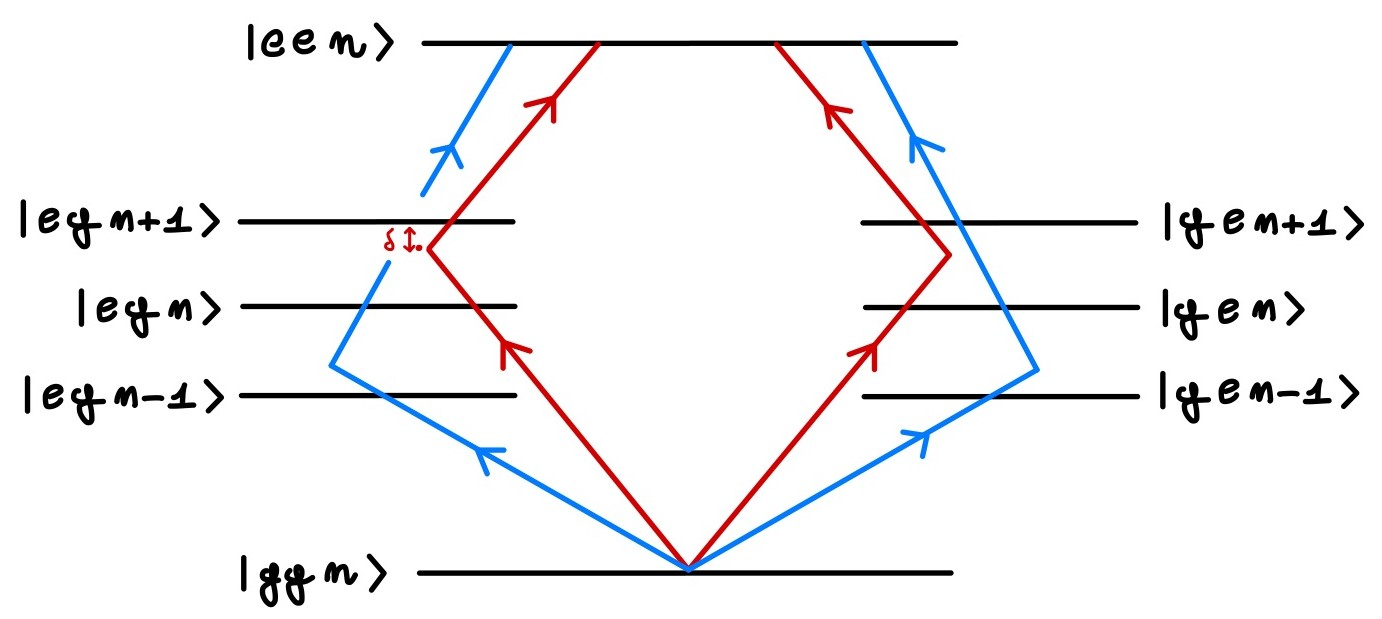
\includegraphics[scale=.31,keepaspectratio]{images/molmer_sorensen1}} \\
	\subfloat[][\label{subfig:molmer_sorensen2} ]{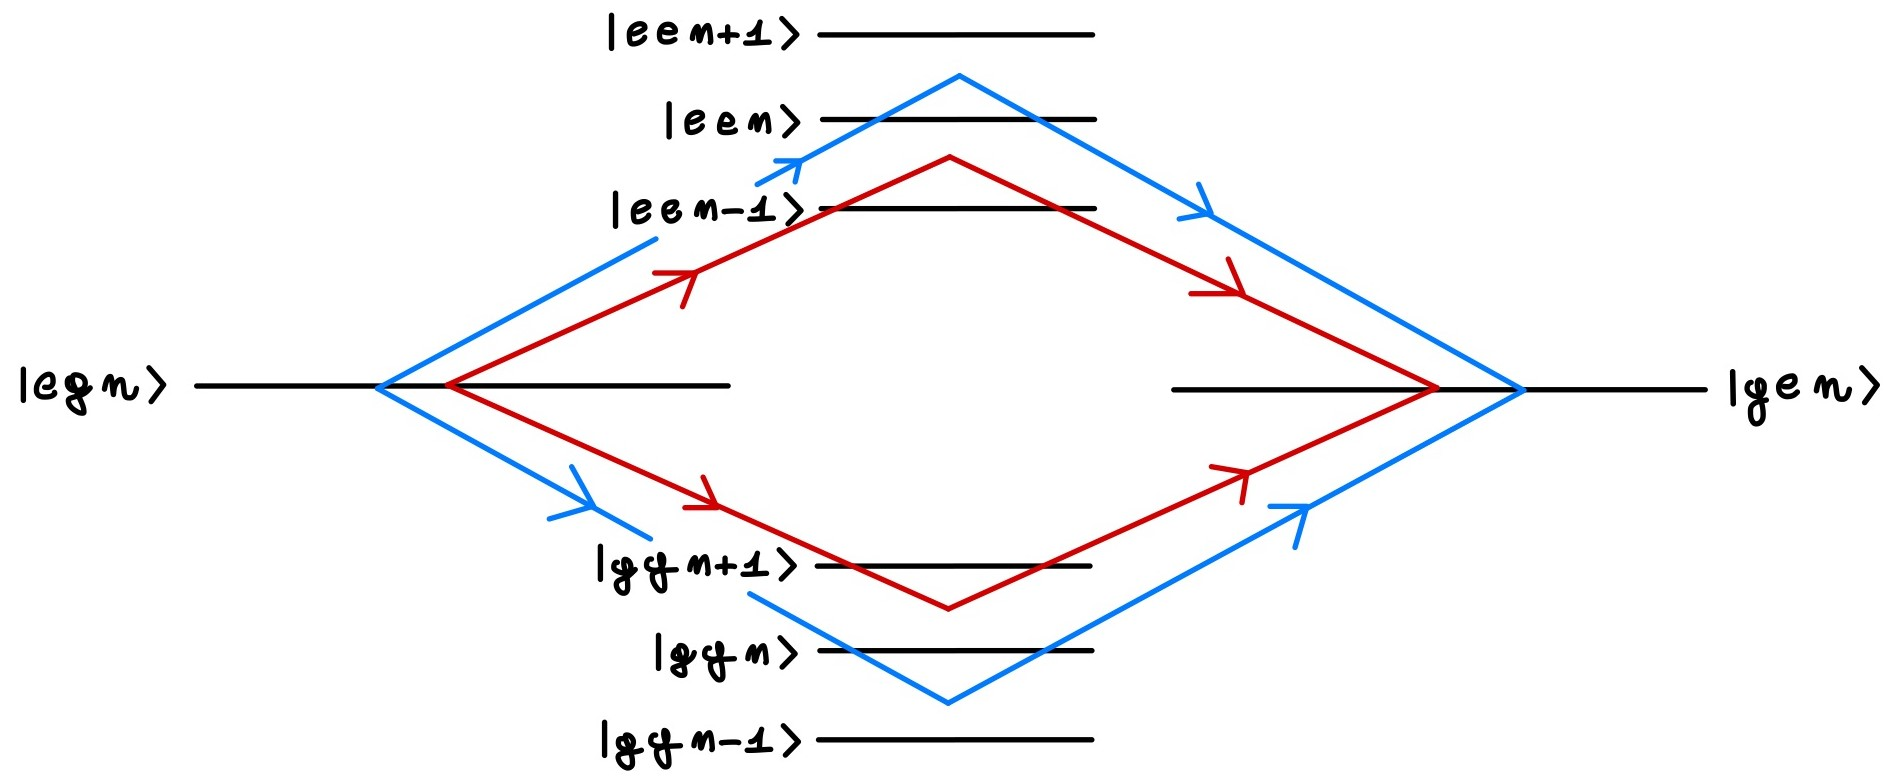
\includegraphics[scale=.31,keepaspectratio]{images/molmer_sorensen2}}
	\caption{(\ref{subfig:molmer_sorensen1}) Oscillazioni di Rabi che connettono gli stati $\ket{ggn} \leftrightarrow \ket{een}$ nel M\o lmer-S\o rensen gate. (\ref{subfig:molmer_sorensen2}) Caso analogo al precedente in cui sono connessi gli stati $\ket{egn} \leftrightarrow \ket{gen}$.}
    \label{fig:molmer_sorensen}
\end{figure}

\noindent Come mostrato in Figura \ref{subfig:molmer_sorensen2}, lo stesso setup può essere utilizzato per connettere gli stati $\ket{egn} \leftrightarrow \ket{gen}$: è quindi possibile, in generale, creare oscillazioni di Rabi tra gli stati $\ket{ggn} \leftrightarrow \ket{een}$ e $\ket{egn} \leftrightarrow \ket{gen}$. 

\noindent Questa tipologia di trasformazioni sono al secondo ordine in teoria delle perturbazioni: gli stati intermedi non sono mai realmente popolati perché per poter effettuare operazioni sui qubit per mezzo delle oscillazioni di Rabi è necessario lavorare alla risonanza. In generale questo non è del tutto ovvio, tuttavia la cosa molto ingegnosa sta nel fatto che le oscillazioni di Rabi risultanti sono del tutto indipendenti dal numero $n$ di fononi! Dunque non è più necessario raffreddare il sistema. 

\noindent Per mostrarlo rigorosamente è necessario svolgere un conto completo in teoria delle perturbazioni dipendenti dal tempo. Intuitivamente si può notare che, dato che $\hat{H}_{\text{int}} \sim (\hat{a} + \hat{a}^\dag)$, allora negli stati dei modi vibrazionali si possono avere solamente un fonone in più o un fonone in meno rispetto allo stato di partenza, quindi $\ket{m} = \ket{n+1}$ oppure $\ket{m} = \ket{n-1}$; ciò è dato dal fatto che solamente gli elementi di matrice di questi stati intermedi sono diversi da zero, ossia $\mel{n}{\hat{a}}{n+1} = \sqrt{n+1}$ e $\mel{n}{a^\dag}{n-1} = \sqrt{n}$. Per questo motivo, un calcolo in teoria delle perturbazioni per campo debole produce  un'ampiezza di Rabi  indipendente da $n$:
\begin{equation*}
    \begin{large}\substack{\text{Ampiezza} \\
    \text{di Rabi}}\end{large} \sim \sum_m \frac{\mel{een}{\hat{H}_{\text{int}}}{m} \mel{m}{\hat{H}_{\text{int}}}{ggn}}{E_m - E_{ggn} - \omega} \sim \frac{(n+1)}{\delta} + \frac{n}{-\delta} \sim \frac{1}{\delta} \, .
\end{equation*}
Un conto pi\`u completo  in approssimazione RWA consente di calcolare esattamente l'operatore di evoluzione temporale che ha la forma
\begin{equation*}
    \hat{U}(t) \sim e^{\alpha(t) \hat{a} + \alpha^\ast(t) \hat{a}^\dag + i S^2_y \beta(t)} \, , \quad \text{dove} \quad S_y = \sigma_1^{(1)} + \sigma_y^{(2)} \, ,
\end{equation*}
dove $\alpha(t)$ e $\beta(t)$ sono due funzioni del tempo calcolabili. Scegliendo i valori del tempo che risolvono l'equazione $\alpha(t) = 0$, l'operatore di evoluzione temporale diventa indipendente dagli oscillatori associati ai fononi e produce un gate universale che realizza l'entanglement tra due qubit.